\chapter{Experimental setup}\label{sec:twod_setup}
%
	\subsection{Reference Discharge}\label{sec:reference_dis}
%
		\begin{figure}[b!]
			\centering
			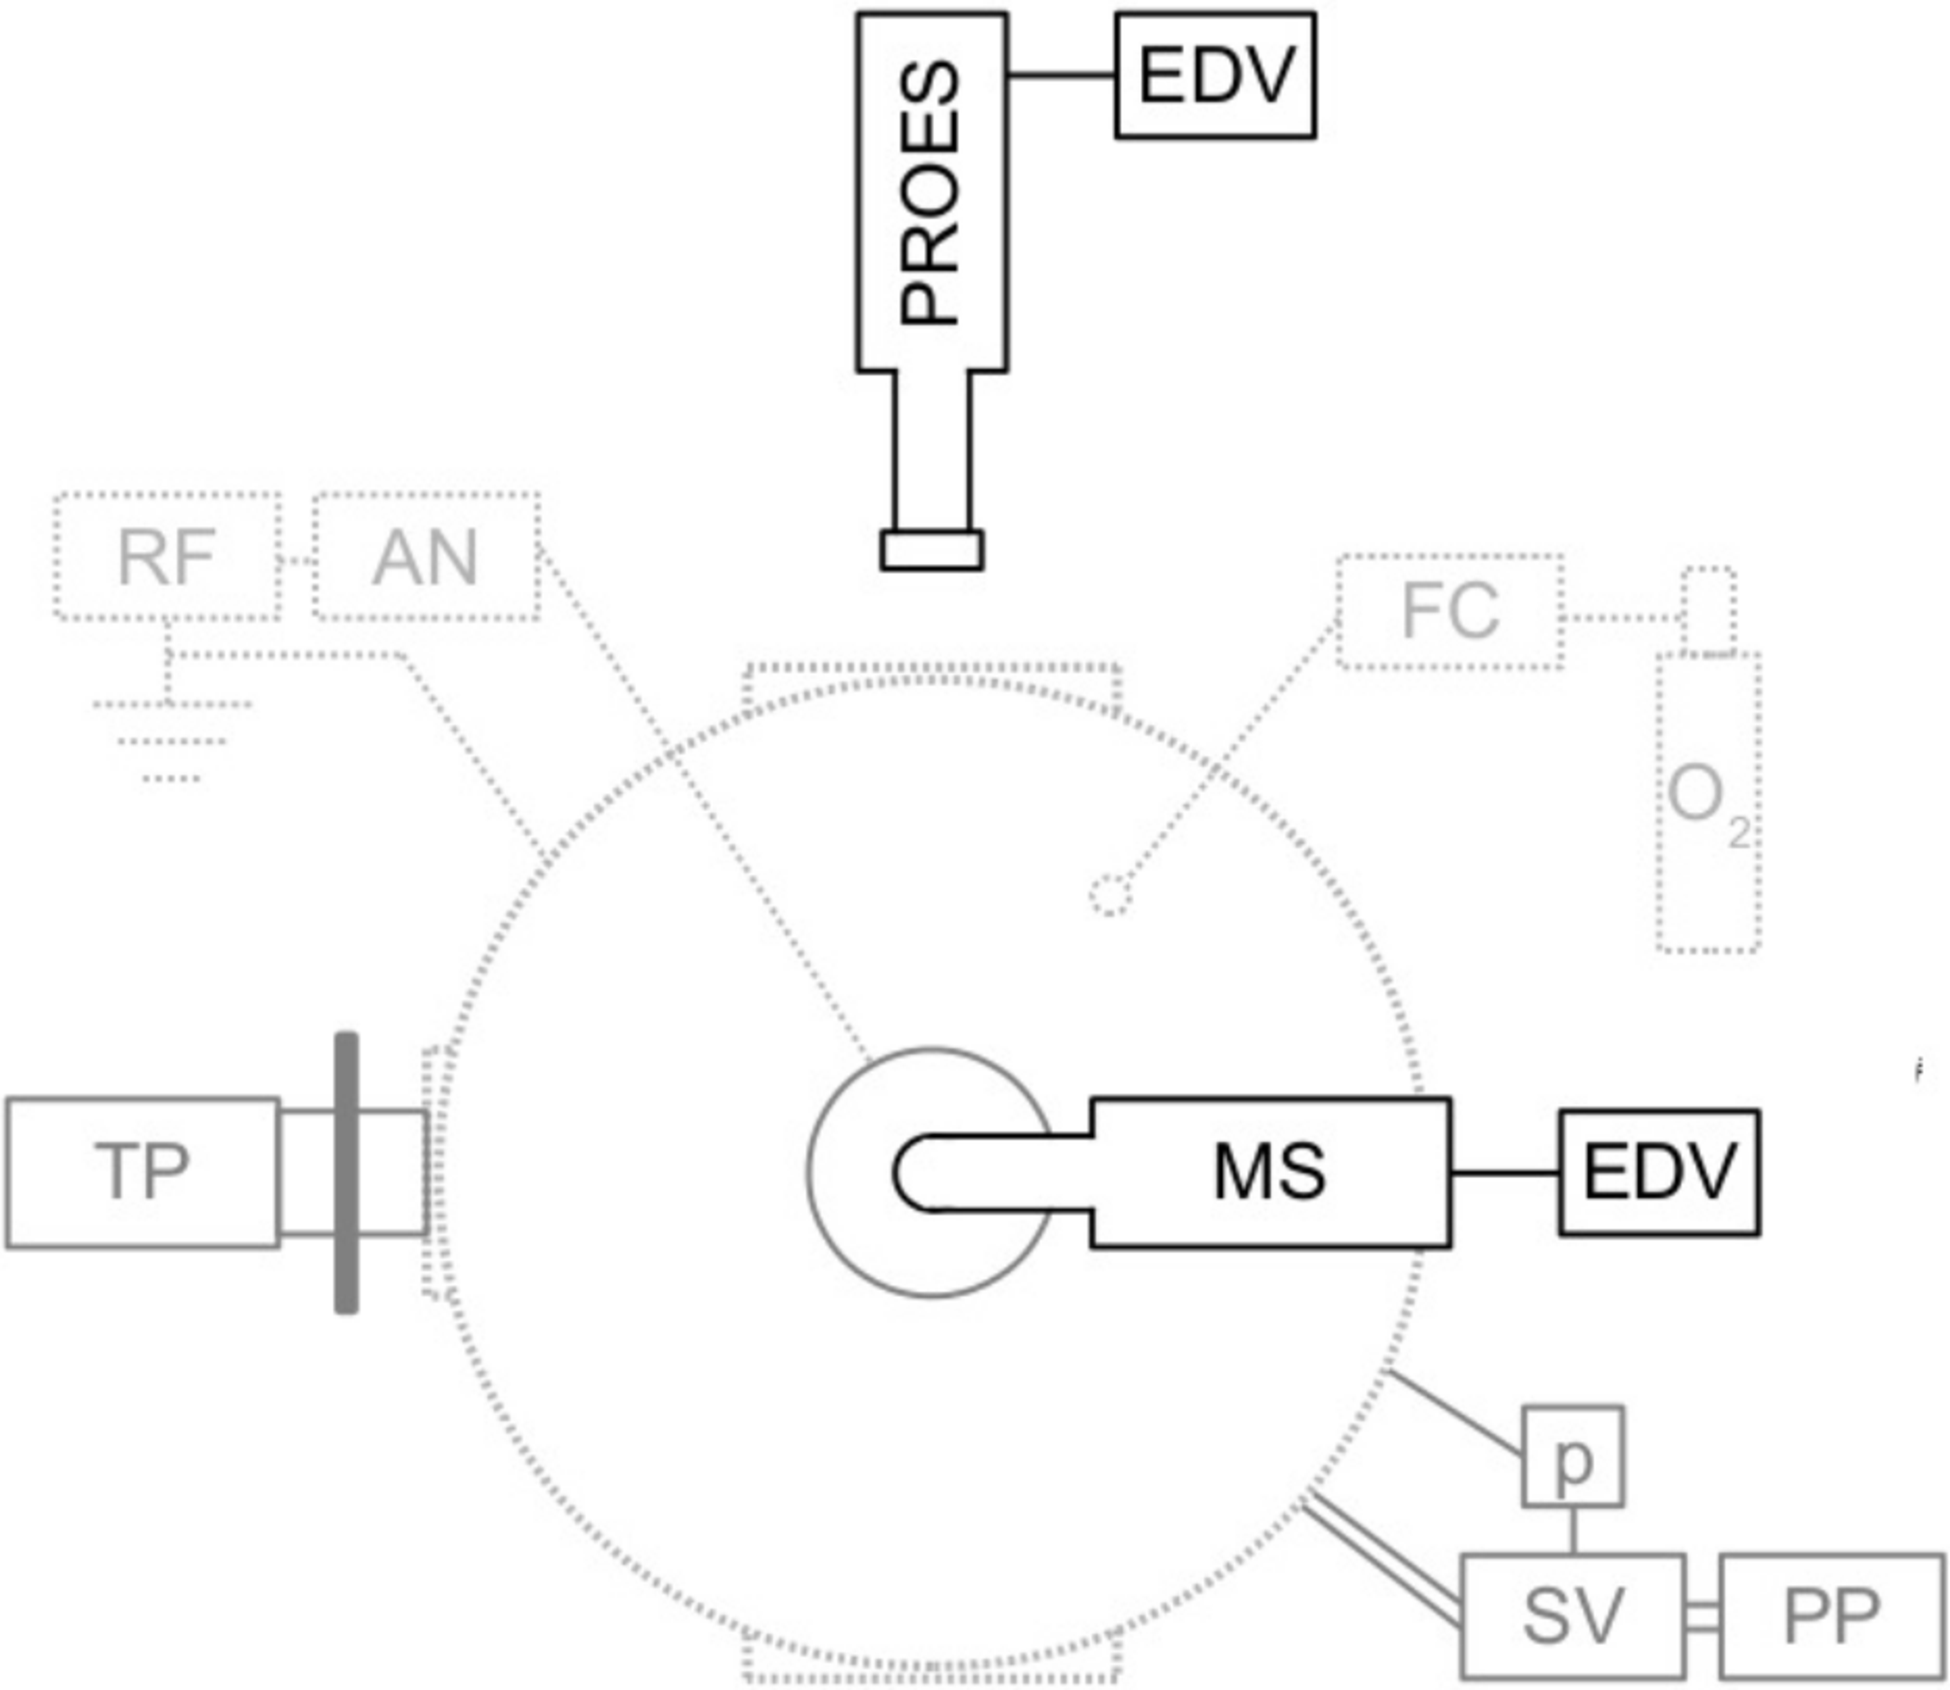
\includegraphics[width=0.5\textwidth]{figures/chamber_exp.pdf}
			\caption{%
				Top-down view schematic of the experiment~\cite{Scheuer15},~\cite{Kullig12}. Shown is the setup %
				without microwave interferometer, like it was used by Küllig et al.}\label{fig:discharge_chamber}
		\end{figure}
%
		Here, the referenced experiment was used by Küllig et al.~\cite{Kullig12} and Scheuer~\cite{Scheuer15}, and consists of a cylindrical setup, filled with oxygen at low pressures and gas flow rates (see~\autoref{fig:discharge_chamber}). The stainless steel vacuum chamber has a diameter and height of $\unit[40]{cm}$ respectively and was filled with the process gas oxygen (O$\ix{2}$) at $\unit[5]{sccm}$ (\fett{FC}). The discharge configuration consisted of an electrode in the centre with $\unit[10]{cm}$ of diameter and a rf generator, constantly operating at a frequency of $\unit[13,56]{MHz}$ and power outputs between $5$ and $\unit[150]{W}$ (\fett{RF} and \fett{AN}), leading to applied voltages in the range of $100$--$\unit[1500]{V}$. Shielding and discharge enclosure/chamber walls are grounded, therefore yielding a large area ratio between driven and grounded electrode and establishing a heavily asymmetric plasma. In addition, the powered electrode was coupled capacitively with the external generator. The value of $U\ix{sb}$ the self bias voltage ranged, depending on power output and discharge pressure, from $-100$ up to $\unit[500]{V}$. In~\cite{Kullig12} the experiment was pulsed with short discharges at a frequency of $\unit[10]{Hz}$. Line integrated measurements resulted in an average electron density of around $\tenpo{11}$--$\unit[\tenpo{12}]{cm^{-3}}$. Showing a schematic top-down view of the experiment is~\autoref{fig:discharge_chamber}. Here, the large ratio between driven and grounded parts is very well visualised. In later simulations it will be of sufficient accuracy to restrain model volume to a smaller setup.\\
		The figure below includes further diagnostics like a mass spectrometer (\fett{MS}) and phase resolved optical emission spectroscopy (\fett{PROES}). The latter measured the mentioned densities via line integration across the plasma volume. The MS is a key instrument for the investigation pursued in this thesis, as it also measures particle numbers energy resolved. For example, the ions created via secondary processes in the discharge sheath are accelerated towards the bulk and thus get into the MS with their characteristic speeds and mass. A significant increase of electron density was found for rf powers larger than $\unit[50]{W}$ or $\unit[-220]{V}$ self bias voltage~\cite{Kullig12}. This led to a correlating negative oxygen ion density reduction and decrease of the electronegativity ratio $\overline{n}_{i,-}/\overline{n}\ix{e}$ from $4$ to $0,03$. During a different operation mode --- called $\alpha$-mode, contrary to the afore-mentioned $\gamma$-mode --- at less than $\unit[50]{V}$ output power, electronegativity rises again, as well as the electron temperature $T\ix{e}$, yielding higher rate coefficients for, e.g.\@ dissociative electron attachment and the alike. See~\autoref{sec:anionproduction} for a more detailed approach.
%
	\subsection{Simulated Discharge}\label{sec:simulatedd_dis}
%
	All of the above conditions are sufficient for a practical approach at a labratory ccrf discharge with great repeatability. Though being highly optimised and developed over the course of many years, the two-dimensional particle-in-cell code outlined above does not provide the tools and performance to feasibly simulate such large areas and particle numbers. Hence, one will reducing the numerical burden by simulating smaller discharge areas and average densities, while trying to satisfy the same physical processes exhibited in~\cite{Scheuer15}.\\
	The afore-mentioned 2d3v PIC code is used to simulate the referenced experiment. The spatial dimensions will be the radial component $r$ and axial coordinate $z$. The geometry and simulation is optimised for cylindrical symmetric gas discharges, which has been thoroughly discussed in~\autoref{sec:picsimulationmcc} and~\autoref{sec:pic_2d3v}.\\
		To represent the strong asymmetry between driven and grounded wall areas, the sizes of anode, cathode and grounded chamber parts have been chosen accordingly. The experimental values for the self bias voltage $U\ix{sb}$ were used to create a dc offset on-top of the rf voltage $U\ix{rf}$ at the cathode. The domain composition with cells of width $\lambda\ix{D,e}/2$ (see~\autoref{sec:picbasics}) makes it even more difficult to appropriately model the system. Hence a smaller discharge volume of a $\unit[4,5]{cm}$ radius and an electrode gap of $\unit[2,5]{cm}$ will be simulated. This usually leads to cell counts up to $2\cdot\tenpo{5}$, which is small in comparison to the `real' experiment, which would have to be covered by over $\tenpo{6}$ cells. Furthermore, the numerical expense grows with $N\log(N)$ (see~\autoref{sec:picsimulationmcc}).\\
		One has chosen pressures between $\unit[2]{Pa}$ and $\unit[30]{Pa}$, with the possibility of changing it later during the discharges simulation. The secondary ion emission efficiency was set to $\eta=0,03$, yielding a stable plasma sheath and current into the bulk. In addition, a constant self bias of $\unit[-200]{V}$ was applied at the cathode. The radio frequency was set to $\unit[13,56]{MHz}$.\\
		The governing electron density and temperature were set to $\unit[5\cdot\tenpo{9}]{cm^{-3}}$ and $\unit[5]{eV}$ respectively, which, as an initial value and property for scale, is sufficient for the necessary rate coefficients mentioned above. This led to the following important scales of simulation: 
%
		\begin{align}
			\lambda\ix{D}&=\unit[0,0235]{cm}\,,%
			\hspace*{2.0cm}%
			\omega\ix{p,e}=\unit[3,99\cdot\tenpo{9}]{Hz}%
			\label{equ:debyeandomega}\\[0.0cm]
			\Rightarrow \Delta x&=\frac{1}{2}\,\lambda\ix{D}=\unit[0,01174]{cm}\,,%
			\quad\quad%
			\Delta t=0,2\cdot\omega\ix{p,e}=\unit[5,015\cdot\tenpo{-11}]{s}%
			\label{equ:simulationscales}
		\end{align}
%			
		Thus a single rf cycle at the given frequency takes $1460$ steps, and the domain measures $384$ and $213$ cells in radial and axial dimension respectively. An ion temperature is adjusted via the fraction $T\ix{i}/T\ix{e}=0,008$, hence the corresponding velocities for the previously defined electron temperature $T\ix{e}=\unit[5]{eV}=\unit[5,8\cdot\tenpo{4}]{K}$ are found to be
%
		\begin{align}
			v\ix{th,e}=&\,\unit[9,37\cdot\tenpo{5}]{\frac{m}{s}}\,,%
			\quad\quad%
			c\ix{s,e}=\,\unit[3,87\cdot\tenpo{3}]{\frac{m}{s}}%
			\label{equ:electronvelocities}\\[0.0cm]%
%				IONS 
			v\ix{th,i}=&\,\unit[558,38]{\frac{m}{s}}\,,%
			\hspace*{1.2cm}%
			c\ix{s,i}=\,\unit[371,44]{\frac{m}{s}}%
			\label{equ:ionvelocities}
		\end{align}
%
		\begin{wrapfigure}{r}{0.3\textwidth}
			\centering
			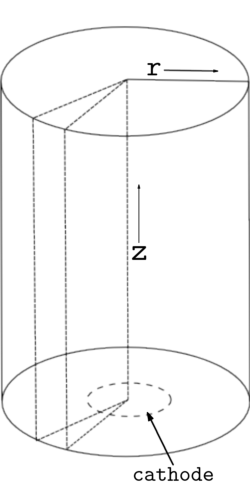
\includegraphics[width=0.275\textwidth]{figures/radial_cylinder.pdf}\\
			\vspace*{0.3cm}\hspace*{0.1cm}
			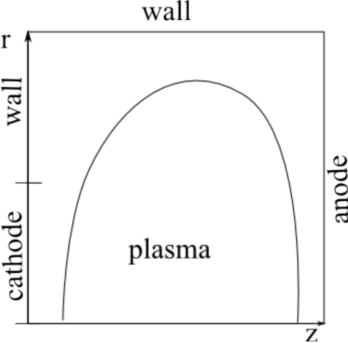
\includegraphics[width=0.275\textwidth]{figures/domain_slice.pdf}
			\caption{%
				Simplified cylinder schematic for the simulated experiment. The slice depicte in the top %
				is shown below. There, boundaries and bulk position are outlined.}\label{fig:radialcylinder}
		\end{wrapfigure}
%
		Here, a single millisecond of operation takes days, if not weeks to simulate with a given timestep, like in~\autoref{equ:simulationscales}. In this case, a single neutral gas particle is statistically amplified by a factor of $\approx 9,3\cdot\tenpo{7}$ to account for the gas density at $\unit[5]{Pa}$ and $\approx\unit[300]{K}$. This number is crucial to all collision processes, where the molecular species O$\ix{2}$ is involved. Charged particle species share a number amplification of $8489$. On top of both super particle factors, a scaling $\sim 1/r$ is applied to consider the variable cell volume.\\
		An assumption in the simulation is a constant neutral gas background. In the experiment, a working gas reservoir and flow rate meter control the pressure and exchange of O$\ix{2}$ inside the chamber. The cold neutral species has a very slow drift velocity, and therefore a large time scale of the transport process in the range of a couple $\unit{ms}$. Also the mean-free-paths are very large and collisions do not change the neutral gas distribution. Hence, the O$\ix{2}$ molecules are initiated at time $t=0$ of the simulation --- this is done with respect to pressure, super particle factor and volume weighting  ---, and are afterwards not altered in number or location. Though collision routines are still exercised, the corresponding movement of the neutral species is not calculated.